
%%%%%%%%%%%%%%%%%%%%%%% file typeinst.tex %%%%%%%%%%%%%%%%%%%%%%%%%
%
% This is the LaTeX source for the instructions to authors using
% the LaTeX document class 'llncs.cls' for contributions to
% the Lecture Notes in Computer Sciences series.
% http://www.springer.com/lncs       Springer Heidelberg 2006/05/04
%
% It may be used as a template for your own input - copy it
% to a new file with a new name and use it as the basis
% for your article.
%
% NB: the document class 'llncs' has its own and detailed documentation, see
% ftp://ftp.springer.de/data/pubftp/pub/tex/latex/llncs/latex2e/llncsdoc.pdf
%
%%%%%%%%%%%%%%%%%%%%%%%%%%%%%%%%%%%%%%%%%%%%%%%%%%%%%%%%%%%%%%%%%%%


\documentclass[runningheads,a4paper]{llncs}

\usepackage{nomencl}
\usepackage{amssymb}
\usepackage{todonotes}
\setcounter{tocdepth}{3}
\usepackage{graphicx}
\usepackage{enumitem}
\usepackage{url}
%\urldef{\mailsa}\path|{alfred.hofmann, ursula.barth, ingrid.haas, frank.holzwarth,|
%\urldef{\mailsb}\path|anna.kramer, leonie.kunz, christine.reiss, nicole.sator,|
%\urldef{\mailsc}\path|erika.siebert-cole, peter.strasser, lncs}@springer.com|    
\newcommand{\keywords}[1]{\par\addvspace\baselineskip
\noindent\keywordname\enspace\ignorespaces#1}
\usepackage[unicode=true]{hyperref}

\begin{document}

\mainmatter  % start of an individual contribution

% first the title is needed
\title{Brain Speed Reader}
%\vspace{1cm}
% a short form should be given in case it is too long for the running head
\titlerunning{Brain Speed Reader}
%\thanks{Please note that the LNCS Editorial assumes that all authors have used
%the western naming convention, with given names preceding surnames. This determines
%the structure of the names in the running heads and the author index.}


% the name(s) of the author(s) follow(s) next
%
% NB: Chinese authors should write their first names(s) in front of
% their surnames. This ensures that the names appear correctly in
% the running heads and the author index.
%
\author{Thomas, Nick, Benjamin, John}


\authorrunning{Thomas, Nick, Benjamin, John}
%% (feature abused for this document to repeat the title also on left hand pages)
%
%% the affiliations are given next; don't give your e-mail address
%% unless you accept that it will be published
\institute{School of Information,\\
UC Berkeley, Berkeley,\\
United States}
%%\mailsa\\
%%\mailsb\\
%%\mailsc\\
%%\url{http://www.springer.com/lncs}
%\and Chair of Entrepreneurial Risks,\\ ETH Zurich, Switzerland}
%
%%
% NB: a more complex sample for affiliations and the mapping to the
% corresponding authors can be found in the file "llncs.dem"
% (search for the string "\mainmatter" where a contribution starts).
% "llncs.dem" accompanies the document class "llncs.cls".
%

%\toctitle{Lecture Notes in Computer Science}
\tocauthor{Authors' Instructions}
\maketitle

\begin{abstract}
At the age of online information abundance, the human capacity to retain knowledge is largely limited by the time and the attention required to read text, watch videos, listen to podcasts. For written information, rapid serial visual presentation (RSVP) helps greatly save time with similar levels of text understanding, compared with traditional reading. However, RSVP does not account for attention. We present a simple hybrid brain-computer interface (BCI) that controls in real-time the speed of reading by measuring the instant level of higher cognitive brain activity. Electroencephalogram (EEG) signal is acquired with a single channel consumer-grade headset and analyzed in the frequency domain. The pace of word display is controlled by a measure brainwave entropy. We have conducted a controlled experiment with 50 subjects with three distinct treatments, and we show that brain-controlled speed-reading increases the speed and the understanding of texts by subjects.
\end{abstract}
\section{Introduction}
Striking the right balance between skimming through newspaper articles, blog posts, tweets, on the one hand, and focusing attention on the most important information contents on the other hand, is an increasingly though challenge in a world of limited time \cite{maillart2011} and attention \cite{anham2006economics}. One way can overcome information overflow by applying filters tailored on individual's past interests \cite{}. This algorithmic approach is however increasingly criticized for generating positive feedback loops and so-called filter bubbles, leaving people exposed to more of the same information \cite{}. Another approach consists in optimizing individual exposure to information, in a way that more knowledge can be processed for the same amount of time.

Speed reading technologies based on rapid serial visual presentation (RSVP) have been developed to increase the throughput of information delivered to people's eyes \cite{slate2014}. {\bf [say more about current speed-reading technologies]}. People choose the speed in their comfort zone (usually around 125 milliseconds per word) prior to reading the text. If the text appears to be harder than expected a slower speed would have been desirable. On the contrary, an easy or boring text, may not deserve as much time, and speed reading could go significantly faster.

Current speed-reading technologies lack the seamless speed control needed to provide online optimization of time spent on each word displayed, or at least on portions of sentences and paragraphs. Interestingly, the wish to seamlessly control RSVP dates back to the very invention of this technique by early cognitive scientists \cite{}.

Brain computer interfaces (BCI) are well-known for being seamless. They have primarily been developed to help heavily motor-impaired recover some communication capabilities, in a way that no physical input is required from the individual \cite{}. Other types of BCI involve neurofeedback, which is used as a remediation technique for people suffering mainly from the Attention Deficit Hyperactivity Disorder (ADHD) \cite{}. Most consumer-grade applications, fostering ``attention" and ``meditation" training using brainwaves rely on similar mechanisms \cite{}.

Controlling speed reading requires however to process signal almost as fast a it is delivered by EEG signal, which is of the order of hundred milliseconds. Moreover, this processing must be lightweight enough to run on a normal computer or mobile device, without slowing the presentation of words on the reader's screen. To enhance usability, the approach should avoid long and boring calibration procedures, and should be efficient from the start.

We address the problem of online optimization of speed reading, with a lightweight algorithm, which guaranties real-time adaption of the rate of word presentation as a function of cognitive activity as captured by single-channel EEG device.

This paper makes 2 primary research contributions: 

(1) It establishes the {\it feasibility} of speed reading system seamlessly controlled by single-channel EEG signal, and 

(2) it exhibits improvements in {\it understanding, comfort and speed} compared to speed reading with constant rate of word display.


%
%The core problem is the time required to actually read, process and memorize information for future restitution, and RSVP was primarily invented for the purpose of studying the fine-grained memory processes at work when people read text \cite{}, listen to audio streams \cite{}, or are presented with images \cite{}. In the case of language, in particular words displayed one after the other, it appears that the time-gains come from reduced eye movement, as the focus remains in a narrow area where the word is displayed \cite{}. Research in cognitive science shows that words can be presented at as fast as XXX words per second without significant loss of understanding and integration (see Section \ref{} for more detailed review of literature, and precisions regarding the nature of understanding and integration: recall, conceptual understanding, etc.). 
%
%Nevertheless, some texts contain words that are most difficult than others, which require extra memory and conceptual processing after each word (resp. group of words). For instance, a short pause at the end of sentences (resp. paragraphs), considerably helps understanding and recall \cite{}. In other words, the capacity to understand a text stems for an adequate optimization (minimization) of time required for integrating knowledge, which might also differ from one subject to another. This optimization can be made manually (i.e., set the number of words per second) at the level of several texts, of one text, maybe at the level of a paragraph, but hardly at the word level, since the time required to set the pace would eliminate the gains obtained from using RSVP. Also, optimization at the text or paragraph levels requires prior knowledge on the text by the user, which is unpractical since the {\it a priori} goal of RSVP is not consolidating knowledge, but rather going quickly through information.
% 
%We are therefore left with three solutions, which consist in (i) setting an average word pace for all words and all text (this average word pace can be manually set/optimized by the user, (ii) programmatically infer the time required to integrate the meaning of a word \cite{smith2013effect}, or (iii) sharply reduce the cost of optimizing the pace-of-word.
%
%The emergence of consumer-grade Brain Computer Interfaces (cBCI) open new opportunities for such seamless and fine-grained control, beyond medical or lab experimentations. Although usual BCIs rely on medical grade devices, we have previously shown the feasibility of cBCI interface with cheap consumer-grade EEG devices, relying on \textcolor{red}{\bf [complete sentence here]} \cite{}. We shall expand this method, using a continuum of entropy-based attention metrics, to compute in real-time the level of attention around each word presented and control the pace of words accordingly, in a continuous optimization process.
%
%


\section{Related Work}
\label{related_work}
Rapid serial visual presentation (RSVP) has been one of the most used techniques for understanding online cognitive processes, and for designing efficient brain-controlled interfaces (BCI), including widely investigated BCI virtual keyboards \cite{}. Research on cognition intersects with techniques to analyze electroencephalogram (EEG) in the time and frequency domains, in particular, when considering the processing of language \cite{}. 

\subsection{RSVP and Cognition}
In cognitive sciences, rapid serial visual presentation (RSVP) has been developed as a way to control the rate of stimuli appearance, in a sequence of words or pictures. Varying stimuli and their rate of appearance helped {\it reverse-engineer} and as a result, understand better how the brain first processes information presented before the subject eyes, and then help recall it. Typical tasks include asking a subject to recall world lists of varying length and presented at varying rates. Results show that recall performance is not only a (negative) function of wordlist length and presentation rate \cite{}, but also a positive function of word congruence \cite{}: if words in the list are more related to each others, then they are altogether easier to recall \cite{}. Also, the way stimuli are recalled count: if the restitution is exactly the input, there is a good chance that  short-term working memory (STM) has been solicited \cite{}. On the contrary, if the restitution is not exactly like the input, but makes use of conceptually close words or images, then these concepts are likely to be pulled out a long-term memory (LTM). Some additional types of memory have been identified, such conceptual short-term memory (CSTM), which acts as buffer between STM and LTM \cite{potter1993very}. The relations between these different memory types and their respective latencies have concrete implications on the understanding of natural language sequences of words \cite{potter1984rapid}. For example, a short time latency after a sentence or paragraph usually improves knowledge integration \cite{see review by potter}. Also, the time required to reading a series of words in natural language can be estimated at the word level as being logarithmic of the word predictability, which is itself related to word congruence in the text \cite{smith2013effect}. \textcolor{red}{\bf [I am still missing some references on the processing lag (between stimulus and conceptualization ($~200ms$?]}

Potter et al. (1980) found RSVP to an effective way to ensure every word is read, but less effective than rapid reading when overall retention was measured. It is worth noting that scrolled and rapid serial visual presentation texts are read at similar rates by the visually impaired \cite{fine1995scrolled} \textcolor{red}{\bf [ could be moved to intro or discussion or both]}. Chen (1983) found that the half of his college subjects who were less good readers remember more from RSVP paragraphs than from conventional paragraphs viewed for the same total time; the better readers showed a slight but not significant drop, with RSVP.

\subsection{Neurosciences of Natural Language Processing}
With the development of neuroimaging techniques, such as electroencephalograms (EEG), magnetic resonance imaging (MRI), and functional MRI (fMRI), the study of cognitive processes has become physiological, with improved possibilities to observe brain activations in space and time, following one or multiple stimuli. For instance, neuroimaging of short-term and long-term memory processes has been studied with EEG in the spectral dimension \cite{klimesch1999eeg,khader2011eeg}, and suggest that increased activity within the upper alpha () and theta () frequency bands correlate with search and retrieval processes of semantic information stored in cortical associative networks \cite{klimesch1996memory,klimesch1990alpha}. Results from several studies \cite{khader2011eeg} suggest that upper alpha seems to be related to semantic long-term memory (LTM) retrieval, while theta activity seems to be related to episodic LTM encoding \cite{} and the maintenance of information in short-term working memory \cite{}. 

%EEG alpha and theta oscillations reflect cognitive and memory performance: a review and analysis \cite{klimesch1999eeg}, as well as in relation with short-term and long-term memories.  \cite{khader2011eeg}. 

Language is intimately related to cognitive processes associated with memory, and because it is a feature almost unique human beings, it accounts as one of the most interesting, challenging and highly investigated research topics in neuroscience \cite{beeman1998right,pulvermuller2002neuroscience}. Language has traditionally been attributed to the Broca Region {\bf [say more here from the paper]} \cite{keller2009broca} and, it was found that left prefrontal brain regions are substantially more involved during encoding of verbal stimuli, which is correlated with increased involvement of the semantic memory system and simultaneous encoding into the short-term memory \cite{fletcher1998functiona,tulving1994hemispheric}. Language processing being a complex task, not only one region and particular frequency ranges of the brain are involved. Weiss et al. \cite{weiss2000long} found long-range EEG synchronization during word encoding associated with high memory performance (primarily between the prefrontal and temporal-parietal regions), as well as an increase in spectral activity in the lower frequencies \cite{kujala2007phase}. It was also found that higher frequencies (Gamma range $>20Hz$) exhibit an increased intensity during processing of words \cite{pulvermuller1995spectral}. From EEG studies, it was found that language processing triggers increased neuronal communication in a variety of regions, but importantly in the frontal-parietal region, and over many frequency ranges [$\theta$ (4 to 7 Hz),$\beta_1$ (13 to 18 Hz) and $\gamma$ (30 to 34 Hz)] \cite{weiss2005increased}. A recent RSVP study combined with Magnetoencephalogram (MEG) spatio-temporal acquisition of coherence of brain regions brought evidence that the 8-13 Hz frequency range (followed by 16-24Hz for four over nine subjects) accounts for most signal associated with reading, and across brain regions, with particularly high coherence density {\bf [explain or rephrase this]} in the frontal-parietal region \cite{kujala2007phase}, although a number of other regions appear to be involved with the cognition processed associated with language processing and reading, reflecting the necessary complex cognitive operations associated with a complex interplay of neuronal synchronizations in the spatial and frequency domains.

%(MRI study?) Activation of left prefrontal and medial temporal cortices were engaged during the encoding of both recalled and forgotten words \cite{wagner1998building}. At least partially supported by Kapur et al. \cite{kapur1996neural} in a PET (positron emission tomography) study 

%Processing new and repeated names: Effects of coreference on repetition priming with speech and fast RSVP  (ERP?) \cite{camblin2007processing}

Although language is a complicated and hard to describe from a physiological perspective, there is reasonable support for brain coherence appearing at various frequency ranges, following the complicated cognitive processes, involving short-term and long-term memory.

%o our knowledge, nothing has been done related to language with consumer grade EEG.
%Here, we shall show that existing research work supports the hypothesis that a single EEG channel set on the forehead, can detect useful signal for our purpose, and show that we do is feasible, at least in principle. {\bf [Important parameters : main location of signal, wave frequency, and maybe latency]}. 

\subsection{Brain Computer Interfaces}
The varied yet repeated patterns observed in the brain has provided hope for applications relying on a direct interface between the brain, a processing unit (e.g., a computer), and by extension any system controlled by a computer. Applications involving brain computer interfaces (BCI)  span from neurological rehabilitation \cite{daly2008brain} to neurofeedback \cite{lubar1995evaluation,fuchs2003neurofeedback} to brain-controlled wheelchairs \cite{galan2008brain}, or even steering a fighter jet simulation with a robotic arm controlled through 96 micro electrodes implanted in the brain \cite{BCIfighterJet2015}.

Most current BCI approaches are developed in the lab, and most often for very specific applications involving rehabilitation and remediation, mainly building on the temporal characteristics of the EEG signal, namely event-related potential (ERP) \cite{brouwer2010tactile}. Recent work has however featured results obtained with consumer grade  EEG headsets, which price is of the order of a few hundred dollars. For instance, it has been demonstrated that the signal of a Neurosky Mindset, a single channel dry EEG headset, can be used to improve driver alertness through appropriate music selection, through a drowsiness detector, involving a combination of machine learning techniques \cite{liu2013driverAlertness}. The same Neurosky device may help bring ``passthoughts"  to the consumer market, as a form of two-factor authentication relying on a mental gesture combined with inner biological brain signal \cite{chuang2013ithink}. This passtought approach has recently been further tested and found to be robust against impersonation attacks \cite{jonhson2014mythoughts}. Building on the same approach, Merrill et al. \cite{merrill2015} developed a simple approach for the classification of mental tasks, using logarithmic quantization combined with a progressive calibration technique. Overall, comparison of consumer-grade single channel EEG with research-grade EEG shows that while consumer-grade EEG cannot locate the origin of the signal, it can discriminate well enough variations of power spectrum intensity, and thus, has potential utility for tasks requiring portability and ease of use \cite{johnstone2012eeg}.


%We are aware that our input device is of low quality, and cannot, by design, capture spatial brain activation (there is only one electrode). Also, we assume that the low quality (i.e., one channel with dry EEG) is not sufficient to capture time delays (ERPs), usually observed in response to stimuli \cite{}. 

%\subsection{RSVP, Cognition and Memory}
%Research on cognition relating to a rapid sequence of words \cite{forster1970visual} and pictures \cite{potter1975time,potter1969recognition} go back to the 70's and 80's. RSVP offers a way to control these processes at fine-grained level. Rapid serial visual presentation (RSVP): A method for studying language processing \cite{potter1984rapid} 
%
%
%This research is centered on (i) how long it takes to internalize the meaning of a word or a sentence, sufficiently that it is possible to recall it accurately, (ii) what kinds of memory processes are solicited [short-term memory (STM) or iconic memory, long-term memory (LTM), working memory (WM)], and (iii) how these are engaged to transform ``raw" information into ``conceptual" information, which can be recalled more easy \cite{}. To emphasize on the interplay between STM bringing information, and LTM pulling out useful concepts for broader understanding, Molly Potter introduced Conceptual Short-Term Memory (CSTM) \cite{potter1993very}. ``Unlike STM, CSTM is central to cognitive processing.
%Recognition of meaningful stimuli such as words or objects
%rapidly activates conceptual information and leads
%to the retrieval of additional relevant information from
%LTM." \cite{potter1993very}. It also depends on the goals set: e.g., identify a specific item in a list, or get a conceptual understanding of a sequence.

%It is important to point out the difference between the capacity to recall unrelated words versus semantically related words, but also, in the case of whole paragraphs, some (short) time is required after a sentence to integrate knowledge \cite{}.



%Visual perception of rapidly presented word sequences of varying complexity 

%Temporal limits of selection and memory encoding a comparison of whole versus partial report in rapid serial visual presentation \cite{nieuwenstein2006temporal}

%Rapid serial visual presentation: a space-time trade-off in information presentation \cite{de2000rapid}

%\subsection{Memory and Time to Process Information}
%``When people view or listen to continuous sequences of scenes or
%words, as they do when they look around, read, listen, or watch TV,
%a series of conceptual representations is activated. These rapidly activated
%and equally rapidly forgotten representations are the raw material
%for identification and comprehension of words, pictures, and
%sequences such as a sentence, and indeed for intelligent thought more
%generally. The normal ease with which we understand what we read
%and see around us is based on selective processing that takes place
%much faster than has been supposed in many theories of working and
%short-term memory, leading to the CSTM hypothesis." \cite{potter1999understanding,potter1993very}
%
%``CSTM is a processing and memory system different from early visual (iconic)
%memory, conventional short-term memory (STM), and longer-term
%memory (LTh{) in three important respects: (1) the rapidity with which
%stimuli readr a postcategoricaf meaningful level of representation, (2)
%the rapid struchrring of these representations, and (3) the lack of awareness
%(or immediate forgetting) of inforrration that is not structured
%or otherwise consolidated. Structure-building in CSTM ranges from
%spontaneous grouping of words in lists on the basis of meaning (one
%of the simplest forrrs of conceptual structuring) to linguistic parsing
%and semantic interpretation of sentences and more extended texts
%(examples of highly skilled structuring). Organization or structuring
%of new stimuli enhances memory for them." \cite{potter1999understanding}
%
%A capacity theory of comprehension: individual differences in working memory \cite{just1992capacity}
%
%Individual differences in working memory and reading \cite{daneman1980individual}
%
%``Second, this information is used in various ways, depending on the
%viewer's current goal if the viewer is trying to understand the whole
%sequence (e.9., a sentence), the information is used to discover or build
%a comprehensive structured representation, but if the viewer is trying
%to locate and identify a particular kind of information (as in target
%search), then only a subset of the information is selected." \cite{potter1999understanding}
%
%``processingT. he CSTM hypothesis
%is not only that conceptual information is activated rapidly, but
%also that the initial activation is highly unstable, such that the
%information is deactivated or forgotten within a few hundred
%msec if it is not incorporated into a structure (or selected for
%further processing" \cite{potter1999understanding}
%













\section{Apparatus}
The brain speed-reader is an apparatus, which displays words on a screen at variable $r(t)$, which in turn is read by the user. The reading task triggers a change of brain activity, which can be recorded and analyzed through electroencephalograms (EEG). As our apparatus is conceived for use in a naturalistic environment, we have used, {\it Neurosky Mindwave}, the cheapest consumer-grade EEG headset available for less than \$100 on the market. As shown on Figure \ref{fig:apparatus} and explained step-by-step below, the EEG signal is processed online, in order to adapt the rate of words displayed as function of cognitive activity: if the rate $r$ is too large (resp. too low) at time $t$, then reading triggers more  (resp. less) cognitive activity, which in turn allows reducing (resp. increasing) $r$ at $t+1$. In this section, we explain step-by-step the design of the apparatus in details.

\begin{figure}[!t]
\centering
\includegraphics[width=0.9\columnwidth]{../figures/apparatus.eps}
\caption{Brain speed-reader apparatus: {\bf (a)} Words are displayed and read one after the other at a given rate. {\bf (b)} the EEG signal is recorded through a consumer grade device (here the {\it Neurosky Mindwave}). {\bf (c)} The EEG signal is turned every 0.5 seconds into a power spectrum through a Fourier transform, {\bf (d)} the characteristics of the power spectrum are compressed into a single value characteristic entropy $s$ value. {\bf (e)} A new rate of word display is updated by taking into its current value and $s$. {\bf (f)} The rate of word display is updated accordingly.}
\label{fig:apparatus}
\end{figure}

\subsection{Rate of Word Display}
The principle of {\it Rapid Serial Visual Presentation} (RVSP) applied to text, is precisely to display the words of a text at a controlled rate. However, in most RVSP implementations for text, the rate of word display pre-determined and remains constant. In our implementation, the user first calibrates the brain speed-reader by tuning a comfortable baseline word display rate $r_{baseline} = r(t = 0)$. The operation takes only a few seconds. This is a usual way to proceed when using usual text RVSP applications.

\subsection{Brain Activity as Captured by EEG signal}
Unlike traditional text RVSP, we wish to let the user adapt the rate of word display in real-time, through brain activity as captured by EEG signal, to control for a text becoming suddenly becoming more difficult, or just because the mindset of the user has changed, like sudden focus on an important part of the text (lower rate desired) or, on the contrary, loss of attention (higher rate of word displayed desired).

Because we want our apparatus be usable outside the lab, we have chosen the cheapest consumer-grade EEG scanner, available on the market for less than \$100.

\subsection{EEG Signal Processing}
One way to process the EEG signal, consists in analyzing its spectral properties over a determined period. Here, we take a time window of 0.25 second, which allows us to analyze the frequency domain $0-128Hz$, since the sampling rate of the Neurosky Mindwave is 512 measures per second (i.e., 512 Hz). Hence, every 0.25 second, we compute the power spectrum given by, 

 \begin{equation}
\label{eq:pspectrum}
\mathbf{[pspectrum~here]}
\end{equation}
 
and which is expected to approximately follow a power law, i.e., the probability to find a frequency $x$ is given by the probability density function $pdf(x)  = 1/x^{\mu+1}$. The power spectrum varies as a function of the mental tasks occurring, and potential external perturbations, such as voice, imperceptible and perceptible muscle movements, eye-movement, blinking.


\begin{figure}[!t]
\centering
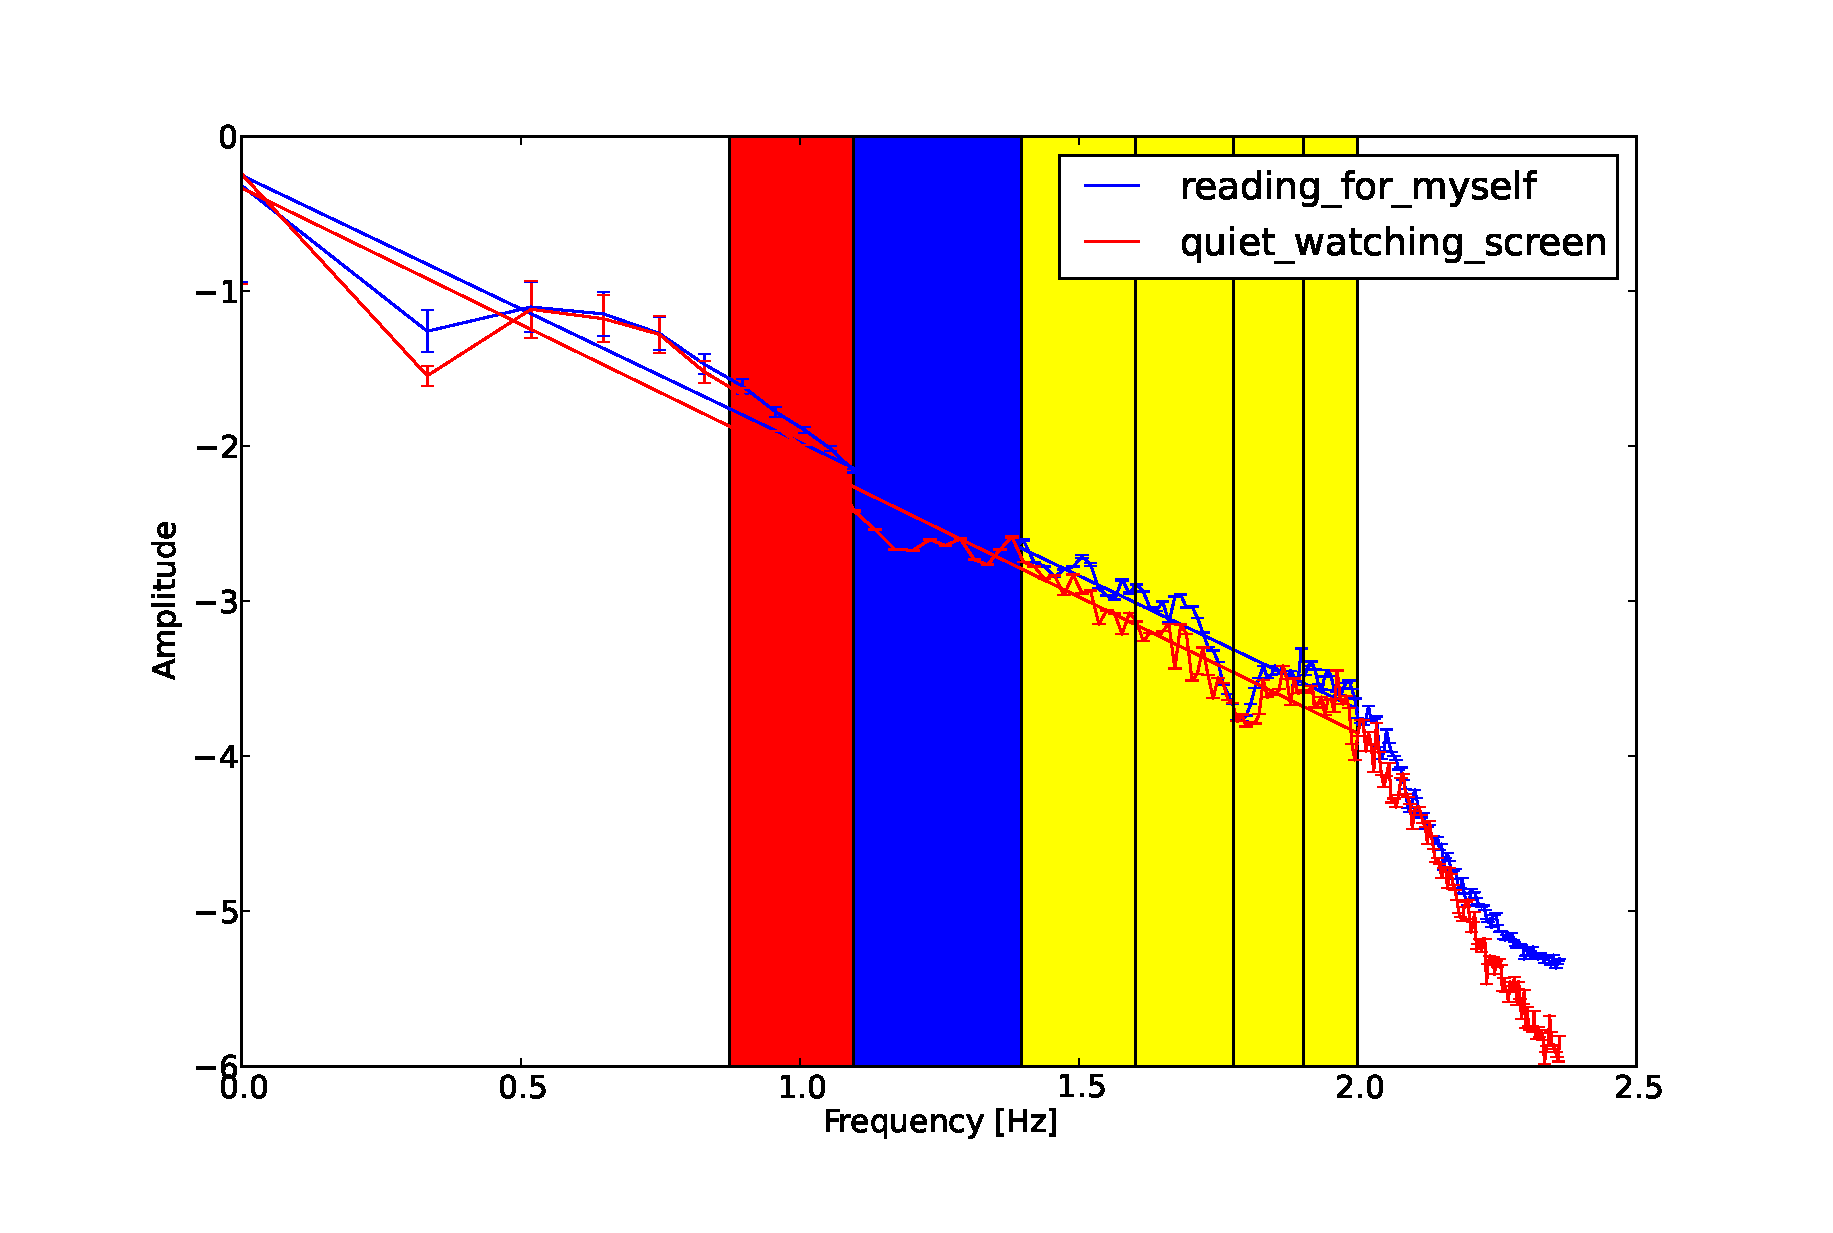
\includegraphics[width=0.9\columnwidth]{../figures/compare_pSpectra.eps}
\caption{Comparison of power spectra of a subject (i) resting state and (ii) reading a text in English for himself. {\bf [report the entropy values in both cases]}}
\label{fig:pspectrum}
\end{figure}


Then, entropy.

\begin{equation}
\label{eq:tsallis}
S_q(X) = \frac{1}{q-1} \left( 1 - \sum_{i=1}^n (p_i)^q \right).
\end{equation}

\begin{equation}
\label{eq:shannon}
S_1(X) = - \sum_{i=1}^n p_i\cdot log_{2}(p_i), ~~for~~q=1.
\end{equation}

\subsubsection{Why Entropy ?}

higher frequencies are usually associated to higher cognitive brain activation. Higher activation  translated into larger entropy $S$.


We wanted a lightweight mobile apparatus, which does not require complicated machine learning or any communication with a cloud service, or would not drain a battery. We purposely decided for a cheap update method {\bf [continue this point in discussion because it helps introduce future work]}

\begin{figure}[!t]
\centering
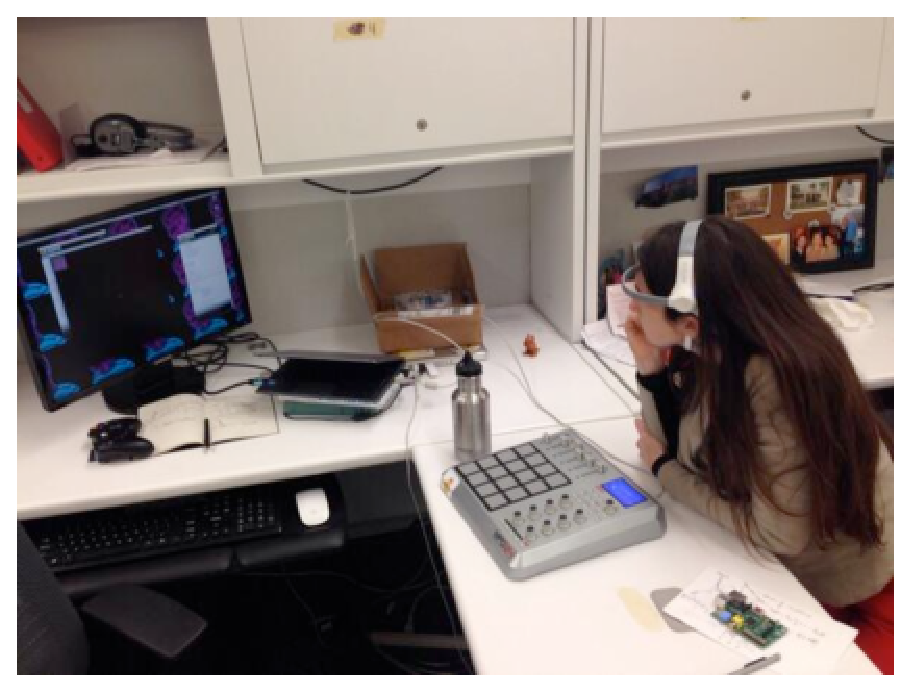
\includegraphics[width=0.9\columnwidth]{../figures/ariel.eps}
\caption{Ariel Garten (Interaxon / Muse CEO) playing with the brain speed reader.}
\label{fig:ariel}
\end{figure}

One could argue that we could have taken the {\it meditation} and {\it attention} metrics provided by Neurosky (and computed directly in the headset). However, these metrics are proprietary and their formula kept secret (we suspect nevertheless that they take $\alpha$ and $\beta$ waves  as an input). Furthermore, extensive testing did not allow us find any consistency with what we would quality meditation or attention. As a result, we preferred to stick to the principles of reproducible science.

\subsection{Negative Feedback Loop}

Explain: higher cog. activity  $\rightarrow$  higher entropy $\rightarrow$  lower word display rate $\rightarrow$ lower cog. activity. {\bf [probably not worth a section]}


\subsection{Word Display Rate Update}

\begin{equation}
\label{eq:Snormalized}
S_{norm}(t) = \frac{S(t) - \langle S \rangle}{\sigma_{S}}, 
\end{equation}
with $\langle S \rangle$ and $\sigma_{S}$ the average and standard deviation of the entropy $S$ calculated over the last 20 points (i.e., the last 5 seconds?). The normalization ensures that $S_{norm}$ is always centered around $0$. The rate $R(t+1)$ of word display is then updated as follows,

\begin{equation}
R(t+\Delta t) = R(t) \left[1 - \alpha \cdot S_{norm}(t)\right],
\label{eq:RateChange}
\end{equation}

where $\Delta t = 0.25$ seconds and $\alpha = 0.20$. In other words, the normalized entropy influences for 20\% the rate change $\Delta R =  \left[ R(t+\Delta t) - R(t) \right] / R(t) = - \alpha \cdot S_{norm}(t)$. Increasing $\alpha$ increases the influence of $S_{norm}$, and the negative sign ensures control of $R$ with a mean reverting process. Note however, that since $S_{norm}$ is calculated from a moving average on a rather short time window, $R$ exhibits excursions (c.f. Figure \ref{fig:trajectory}).

\begin{figure}[!t]
\centering
%\includegraphics[width=0.9\columnwidth]{../figures/apparatus.eps}
\caption{typical evolution of rate $R$.}
\label{fig:trajectory}
\end{figure}

\subsection{Experimental Protocol}
\label{exp_protocol}

To test the research hypotheses proposed in Section \ref{hypo}, and the practical feasibility our {\it brain speed reader} apparatus (c.f., Section \ref{apparatus}), we  have conducted an experiment on XX ($\sim 25$ \textcolor{red}{\bf [30 subjects would be a minimum]}) participants.\footnote{The experimental procedures described here were approved by an Institutional Review Board.} The experimental protocol is as follows, and was conducted on a local web interactive interface, along with the Neurosky Mindwave mobile EEG headset \cite{}.

After obtaining individual consent, we asked each subject to fill general demographics (e.g., age, highest degree obtained), and questions more specific related to reading skills, Attention Deficit Hyperactivity Disorder (ADHD), or any visual impairment that could impede good reading  \textcolor{red}{\bf [we could also try to build a cohort of ADHD]}.

The subject was then asked to perform 4 preliminary tasks presented randomly: (i) resting state for 10 seconds, (ii) eye blink (5 seconds), (iii) watch a short video on screen (30 seconds), and (iv) read a $\approx 500$ words text in silence. For all these tasks, EEG signal was recorded, and in the latter task, reading time was recorded, to establish a benchmark.

The subject was the presented with a list of articles of various topics, length and difficulty (as measured by the ATOS score,\footnote{Michael Milone,The Development of ATOS, The Renaissance Readability Formula, p10 (2010) \url{http://doc.renlearn.com/KMNet/R004250827GJ11C4.pdf} \textcolor{red}{\bf [see if it really makes sense to use ATOS as the main parameters are straightforward, i.e., length of text, words per sentence, characters per word, and average grade level of words (which class grade the word is first seen $\rightarrow$ not necessarily important because we only survey adults]}} borrowed from popular blogs and online news. The subject had to pick 4 articles of her choice for RSVP reading. For each article, one of the four treatments was randomly applied:

\begin{enumerate}
  \item {\bf Constant Rate: } the rate of word display remains constant with $X(t) = X_{0}$ for $\forall t$. The baseline rate $X_{0}$ is determined as 20\% faster than the average time spent by the subject on each word during the text reading preliminary task as described above.
  \item {\bf Brain Speed Reader ($\alpha <0$): } starting from the baseline $X_0$, the rate $X$ changes every quarter second following formula (\ref{eq:RateChange}). This treatment tests {\bf Hypothesis 1a}.
 \item {\bf Brain Speed Reader ($\alpha > 0$): } Similar to treatment 2. Tests {\bf Hypothesis 1b}.
 \item {\bf Randomly Varying Rate: } This treatment mimics the brain speed reader treatment, with a randomly varying $X(t)$, according to an auto-regressive model, calibrated on the same distribution as the random variable$S_{norm}$.
\end{enumerate}

In treatments {2} and { 3}, $|\alpha|$ was set randomly among $\mathrm{A} = \{0.50, 1.00, 2.00 \}\cdot10^{-2}$.

Each treatment is followed by open comprehension questions: such as identification of the main characters and writing a short summary of the article of maximum 500 characters  \textcolor{red}{\bf [find more standardized comprehension questions, if we can]}, by recall questions, such as finding words that have appeared in the text among a list of words. During the four treatments, the subject was wearing the EEG headset, without knowing whether the treatment was involving feedback control by the way of EEG signal. In other word, the subject and no information on the three treatments, and had no possibility to distinguish between these treatments, in other ways than guessing from their experience. At the end, subjects were asked to rank treatments by perceived comfort, understanding, degree of control. We finally, revealed which treatment was associated with each text, we also provided some basic reading performance feedback.

For a subset \textcolor{red}{[$\sim 10$ subjects]}, we repeated the experiment a few hours, days, up to two weeks later, to gain insight on the habituation / learning curve process. \textcolor{red}{\bf [maybe keep acquire these subjects but keep for subsequence publication]}.

%\begin{itemize}
%  \item {\bf text 0 (adapted from Coming of Age in Samoa, Margaret Mead, 1928
%)}:   $ATOS=9.5$,  $word~count = 421$
%  \item {\bf Text 1  (adapted from The Warden, Anthony Trollope, 1855)} : $ATOS=8.3$, $word~count = 563$
%  \item {\bf Text 2  (adapted from The Mayor of Casterbridge, Thomas Hardy, 1886) } : $ATOS=10.2$, $word~count = 831$
%  \item {\bf Text 3 (Adapted from: The Social Function of Science, John D Bernal (1939))} : $ATOS=11.9$, $word~count = 421$
%\end{itemize}


\section{Results}
\label{results}
The {\it brain speed reader} is an attempt to test a fast-paced brain-computer interface, which bets that humans can self-regulate their brain wave modulations, in order to control the rate of stimuli in a rapid serial visual presentation setting. Self-regulation achievement is a token of concentration on the coherent sequence of stimuli displayed. Therefore, to evaluate the {\it brain speed reader}, we have primarily focused on the capacity to self-regulate. We tested two opposed designs: {\it bsr+} ($\alpha = 0.005$) and {\it bsr-} ($\alpha = -0.005$). We compared the brain speed reader treatments to the constant RSVP rate [$X(t)  = 125$ ms/word], for perceived comfort and comprehension, keeping in mind that speed reading, and RSVP speed reading in particular, are somewhat unusual: In our 21 participants sample, only one had practiced speed reading before taking the experiment.

\subsection{Self-regulation achievement \& perceived comfort}
With no previous research or preliminary results at hand, we had no {\it a priori} hypothesis on whether users can achieve self-regulation ($stability <  2$) at all, for both treatments  {\it bsr+} and {\it bsr-}, or only for one of them. We found that 72\% of the participants who took {\it bsr+} achieved self-regulation at least once. Similarly, 58\% of the participants could achieve self-regulation at least once in the {\it bsr-} treatment. These results show that capabilities by humans to achieve self-regulation are high even without prior training. Self-regulation with {\it bsr+} treatment appears to be only slightly more prevalent, suggesting that one RSVP rate update method is easier than the other. To confirm this hypothesis, we considered participants who achieved self-regulation for both {\it bsr+} and {\it bsr-}. We found that 47\% of the participants could self-regulate with both opposed treatments. This result suggests in turn that, for roughly half users tested, the brain has enough plasticity to adapt the brain wave modulations, in order to successfully control the RSVP rate. Since there is no {\it ex-ante} training in the experiment, we can assert that this adaptation occurs quickly, reflecting a form of brain dynamical plasticity.


\begin{table}[h!]
	\centering
	\caption{Ordinary least square regression of stability.}
	\begin{tabular}{lcccc} \hline
		& (1) & (2) \\%& (3) & (4) \\
		VARIABLES & -Stability & -Stability \\%& $V_{it}$ & $V_{it}$ \\ \hline
		&  &  \\%&  &  \\
		Age & {\bf -0.0300**} & {\bf -0.0345**} \\ %& -2.310*** & -1.236** \\
		& {\it (0.0073)} & {\it (0.0087)} \\%& (0.603) & (0.515) \\
		Normal Read Rate & {\bf 0.1650*} & {\bf 0.0920*}  \\%& -23.72*** & -7.188** \\
		& {\it (0.0628)} & {\it (0.067)} \\%& (2.152) & (3.473) \\
		Text Length & {\bf -0.0013***} &  {\bf -0.0012***} \\%& -3.312*** & -3.758*** \\
		& {\it (0.0004)} & {\it (0.0005)} \\%& (1.239) & (1.128) \\
		Reading Pleasure & {\bf 0.3034*} & {\bf 0.2436*} \\ %& -0.0312 & -0.0321* \\
		& {\it (0.0591)} & {\it (0.0650)} \\ 
		Speed Reading Comfort & {\bf -0.0726*}  & {\bf -0.1217*} \\%& 0.106** & 0.0755* \\
		& {\it (0.0355)} & {\it (0.0346)}  \\%& (0.0431) & (0.0406) \\
		Familiar Topic & {\bf -0.091*} &  \\%& 16.75*** & -7.414 \\
		& {\it (0.040)} & \\%& (1.339) & (5.698) \\
		Constant & -1.3213 & -0.6579 \\%& 190.3*** & 136.5*** \\
		& {\it (0.5390)} & {\it (0.5565)} \\%& (23.17) & (26.17) \\
		&  &  \\%&  &  \\
		
		R-squared & 0.8148 & 0.8930 \\%& 0.319 & 0.647 \\
		p-value & 0.0042 & 0.0083\\
		Observations & 14 & 14 \\%& 1,212 & 1,212 \\
		%Program FE & No & No \\%& No & Yes \\ \hline
		&  &  \\
		\hline
		\multicolumn{3}{l}{ Robust standard errors in parentheses} \\
		\multicolumn{3}{l}{ *** p$<$0.001, ** p$<$0.01, * p$<$0.05} \\
	\end{tabular}
	\label{tab:reg}
\end{table}

We have considered an arbitrary threshold for stability ($stability < 2$), but stability is a continuous variable from 0 (perfect stability, i.e., constant rate) to $\infty$ [here, $max(stability) = 5$ by convention, see section Methods]. Considering participants who achieved stability ($ 0 < stability < 2$), we take stability as a dependent variable, and using a ordinary least square (OLS) model we have investigated which demographic, text, and reported comfort control variables best influence stability (c.f. Table \ref{tab:reg}). We found that reading speed in normal setting, familiarity with the topic, and reading pleasure are highly associated with increased stability. On the contrary, age and text length negatively influences stability achievement. Surprisingly, speed reading comfort and familiarity with the topic (as reported by participants) is also negatively associated with stability. The negative impact of speed reading comfort may suggest that less stability introduces some additional degree of freedom on how users control the RSVP rate (yet at the expense of reading pleasure). We have no explanation for the negative impact of topic familiarity. We have tested a second model (2) by removing the familiarity with the topic. All other parameters remain almost unchanged.

\subsection{Reading speed}
Reading speed is another important factor. During the preliminary tasks, participants were asked to read an article excerpt entirely displayed on the screen. We find that it took $240\pm50$ milliseconds/word to read this piece of text, even though there were no follow-up comprehension questions, unlike for the RSVP treatments for which participants were informed of a detailed description of follow-up comprehension questions. For those who achieved stability during {\it bsr+} and {\it bsr-} treatments, the average RSVP rate was found to be very close to 125 milliseconds per word with 5th and 95th percentiles, respectively 110  and 142 ms/word. The confidence interval of average RSVP rate found here is similar but smaller than what was found as the comfort zone in previous research (80 to 200 ms/word) \cite{kujala2007phase}. Another explanation would be that the proximity of the average RSVP rate with the initial rate $X(t=0) = 125$, may explain why the average rate was found to be very close to this value. 

\subsection{Comprehension}
Now we turn to reading comprehension as tested from (i) short summary, (ii) free recall of proper nouns, and (iii) selecting common nouns. We find limited support suggesting that more stability increases the capacity to produce a meaningful summary (Spearman correlation $\rho= 0.35$, $p = 0.069$). However, we found no effect on proper and common nouns recall.

\section{Discussion}
\label{discussion}


\subsubsection{Summary of results}

\subsubsection{Reconnect with previous results obtained in cognitive neuro-sciences}

\subsubsection{Neurofeedback}
30. Heinrich, H., Gevensleben, H. \& Strehl, U. Annotation: neurofeedback - train
your brain to train behaviour. J. Child Psychol. Psychiatry 48, 3�16 (2007).

\textcolor{red}{\bf [maybe this should be left for a subsequent iteration involving subjects repeating the experiment.]}


Comment by a participant (Tap): ``It would be great to have a way to track eyes, so that when the user attention leaves the screen, the brain speed reader stops"




\subsubsection{Other media}
- audio

- cartoons

- etc.

\subsection{Curing Diseases}
- visual impairment

- adhd



\input{../sections/future_work}

\bibliographystyle{abbrv}
%\bibliography{bib/tmaillart.bib,bib/references.bib}


\end{document}
